\documentclass[journal,12pt,twocolumn]{IEEEtran}

\usepackage{setspace}
\usepackage{gensymb}

\singlespacing


\usepackage[cmex10]{amsmath}

\usepackage{amsthm}

\usepackage{mathrsfs}
\usepackage{txfonts}
\usepackage{stfloats}
\usepackage{bm}
\usepackage{cite}
\usepackage{cases}
\usepackage{subfig}

\usepackage{longtable}
\usepackage{multirow}

\usepackage{enumitem}
\usepackage{mathtools}
%\usepackage{steinmetz}
\usepackage{tikz}
\usepackage{circuitikz}
\usepackage{verbatim}
%\usepackage{tfrupee}
\usepackage[breaklinks=true]{hyperref}

\usepackage{tkz-euclide}

\usetikzlibrary{calc,math}
\usepackage{listings}
    \usepackage{color}                                            %%
    \usepackage{array}                                            %%
    \usepackage{longtable}                                        %%
    \usepackage{calc}                                             %%
    \usepackage{multirow}                                         %%
    \usepackage{hhline}                                           %%
    \usepackage{ifthen}                                           %%
    \usepackage{lscape}     
\usepackage{multicol}
\usepackage{chngcntr}

\DeclareMathOperator*{\Res}{Res}

\renewcommand\thesection{\arabic{section}}
\renewcommand\thesubsection{\thesection.\arabic{subsection}}
\renewcommand\thesubsubsection{\thesubsection.\arabic{subsubsection}}

\renewcommand\thesectiondis{\arabic{section}}
\renewcommand\thesubsectiondis{\thesectiondis.\arabic{subsection}}
\renewcommand\thesubsubsectiondis{\thesubsectiondis.\arabic{subsubsection}}


\hyphenation{op-tical net-works semi-conduc-tor}
\def\inputGnumericTable{}                                 %%

\lstset{
%language=C,
frame=single, 
breaklines=true,
columns=fullflexible
}
\begin{document}


\newtheorem{theorem}{Theorem}[section]
\newtheorem{problem}{Problem}
\newtheorem{proposition}{Proposition}[section]
\newtheorem{lemma}{Lemma}[section]
\newtheorem{corollary}[theorem]{Corollary}
\newtheorem{example}{Example}[section]
\newtheorem{definition}[problem]{Definition}

\newcommand{\BEQA}{\begin{eqnarray}}
\newcommand{\EEQA}{\end{eqnarray}}
\newcommand{\define}{\stackrel{\triangle}{=}}
\bibliographystyle{IEEEtran}
\providecommand{\mbf}{\mathbf}
\providecommand{\pr}[1]{\ensuremath{\Pr\left(#1\right)}}
\providecommand{\qfunc}[1]{\ensuremath{Q\left(#1\right)}}
\providecommand{\sbrak}[1]{\ensuremath{{}\left[#1\right]}}
\providecommand{\lsbrak}[1]{\ensuremath{{}\left[#1\right.}}
\providecommand{\rsbrak}[1]{\ensuremath{{}\left.#1\right]}}
\providecommand{\brak}[1]{\ensuremath{\left(#1\right)}}
\providecommand{\lbrak}[1]{\ensuremath{\left(#1\right.}}
\providecommand{\rbrak}[1]{\ensuremath{\left.#1\right)}}
\providecommand{\cbrak}[1]{\ensuremath{\left\{#1\right\}}}
\providecommand{\lcbrak}[1]{\ensuremath{\left\{#1\right.}}
\providecommand{\rcbrak}[1]{\ensuremath{\left.#1\right\}}}
\theoremstyle{remark}
\newtheorem{rem}{Remark}
\newcommand{\sgn}{\mathop{\mathrm{sgn}}}
\providecommand{\abs}[1]{\left\vert#1\right\vert}
\providecommand{\res}[1]{\Res\displaylimits_{#1}} 
\providecommand{\norm}[1]{\left\lVert#1\right\rVert}
%\providecommand{\norm}[1]{\lVert#1\rVert}
\providecommand{\mtx}[1]{\mathbf{#1}}
\providecommand{\mean}[1]{E\left[ #1 \right]}
\providecommand{\fourier}{\overset{\mathcal{F}}{ \rightleftharpoons}}
%\providecommand{\hilbert}{\overset{\mathcal{H}}{ \rightleftharpoons}}
\providecommand{\system}{\overset{\mathcal{H}}{ \longleftrightarrow}}
	%\newcommand{\solution}[2]{\textbf{Solution:}{#1}}
\newcommand{\solution}{\noindent \textbf{Solution: }}
\newcommand{\cosec}{\,\text{cosec}\,}
\providecommand{\dec}[2]{\ensuremath{\overset{#1}{\underset{#2}{\gtrless}}}}
\newcommand{\myvec}[1]{\ensuremath{\begin{pmatrix}#1\end{pmatrix}}}
\newcommand{\mydet}[1]{\ensuremath{\begin{vmatrix}#1\end{vmatrix}}}
\numberwithin{equation}{subsection}
\makeatletter
\@addtoreset{figure}{problem}
\makeatother
\let\StandardTheFigure\thefigure
\let\vec\mathbf
\renewcommand{\thefigure}{\theproblem}
\def\putbox#1#2#3{\makebox[0in][l]{\makebox[#1][l]{}\raisebox{\baselineskip}[0in][0in]{\raisebox{#2}[0in][0in]{#3}}}}
     \def\rightbox#1{\makebox[0in][r]{#1}}
     \def\centbox#1{\makebox[0in]{#1}}
     \def\topbox#1{\raisebox{-\baselineskip}[0in][0in]{#1}}
     \def\midbox#1{\raisebox{-0.5\baselineskip}[0in][0in]{#1}}
\vspace{3cm}
\title{EE5609 Assignment 3}
\author{KOLLI RAVI, EE20MTECH11017}
\maketitle
\newpage
\bigskip
\renewcommand{\thefigure}{\theenumi}
\renewcommand{\thetable}{\theenumi}
\section{Problem}
$ AD $ is the median of a $\Delta ABC $ and $ AM \perp BC $. prove that \\
$ AB^2 = AD^2 - BC.DM + (\frac{BC}{2})^2 $
\section{Solution}
In a right angle triangle, square of the hypotenuse is equal to the sum of the squares of the other two sides. Also, a medain devides the sides into two  equal halves.\\ 
\renewcommand{\thefigure}{1}
\begin{figure}[hb]
	\centering
	\centering
	\resizebox{\columnwidth}{!}{\documentclass{article}
\documentclass{pgfplots}


\usepackage{tikz}

\begin{document}
\begin{center}
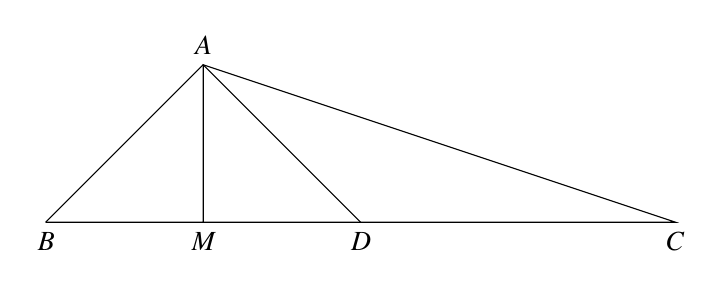
\begin{tikzpicture}

\draw (0,0) node[anchor=north]{$B$}
-- (4,0)  node[anchor=north]{$D$}
-- (8,0) node[anchor=north]{$C$}
-- (2,2) node[anchor=south]{$A$}
-- (2,0) node[anchor = north]{$ M $}
-- (0,0);
\draw (2,2) -- (4,0);
\draw (2,2) -- (2,0);
\draw (0,0) -- (2,2);



\end{tikzpicture}
\end{center}
\end{document}}

\end{figure}

from the above figure\\
\begin{align}
\norm{B-D} = \norm{D-C}
\end{align}

\begin{align}
AM \perp BC
\end{align}
then as per the pythagoras theorem\\
\begin{align}
\norm{A-B}^2 = \norm{B-M}^2 + \norm{A-M}^2
\end{align}
\begin{align}
 = \norm{B-M}^2 + \norm{A-D}^2 - \norm{M-D}^2
\end{align}
\begin{align}
=\brak{\norm{B-D}-\norm{M-D}}^2 + \norm{A-D}^2 - \norm{M-D}^2
\end{align}
\begin{multline}
=\norm{B-D}^2 + \norm{M-D}^2 - 2\norm{B-D}\norm{M-D}+\norm{A-D}^2 - \norm{M-D}^2
\end{multline}
\begin{align}
=\norm{B-D}^2 - 2\norm{B-D}\norm{M-D}+\norm{A-D}^2
\end{align}
\begin{align}
=\norm{A-D}^2 + \norm{\frac{B-C}{2}}^2 - 2 \norm{B-D}\norm{M-D}
\end{align}
\begin{align}
=\norm{A-D}^2 + \norm{\frac{B-C}{2}}^2 - 2 \norm{\frac{B-C}{2}}\norm{M-D}
\end{align}
\begin{align}
=\norm{A-D}^2 + \norm{\frac{B-C}{2}}^2 - \norm{B-C}\norm{M-D}
\end{align}

\hspace{2cm}     Hence proved.




\end{document}
